\documentclass{article}
\usepackage{tikz}
\usetikzlibrary{arrows.meta,positioning,calc,shapes.geometric}
\pagestyle{empty}
\begin{document}
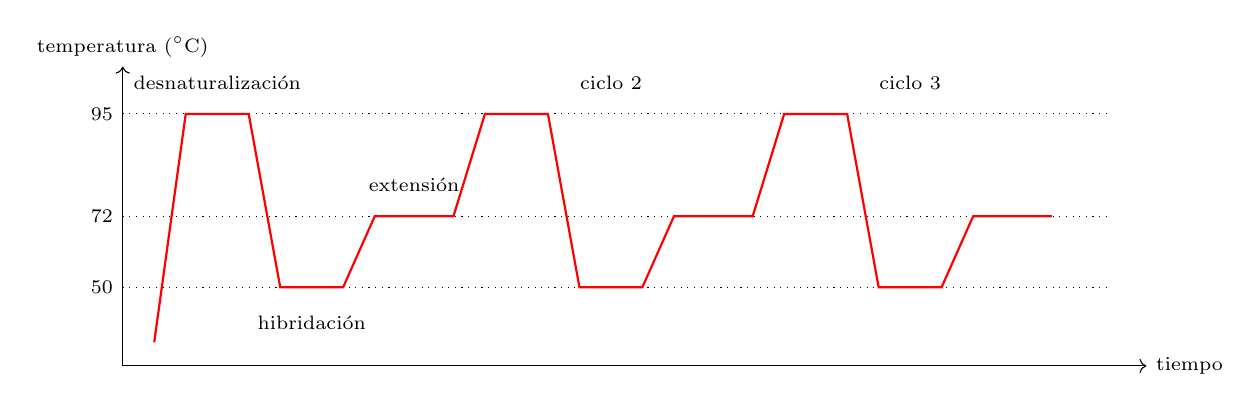
\begin{tikzpicture}

\draw[->] (0,0) -- (0,3.8) node[above, font=\scriptsize] {temperatura ($^\circ$C)}; \draw[->] (0,0) -- (13,0) node[right, font=\scriptsize] {tiempo};
\foreach \t/\y in {50/1.0, 72/1.9, 95/3.2} {\draw[dotted] (0,\y) -- (12.5,\y); \node[font=\scriptsize, left] at (0,\y) {\t};}
\draw[thick, red] (0.4,0.3) -- (0.8,3.2) -- (1.6,3.2) -- (2.0,1.0) -- (2.8,1.0) -- (3.2,1.9) -- (4.2,1.9) -- (4.6,3.2) -- (5.4,3.2) -- (5.8,1.0) -- (6.6,1.0) -- (7.0,1.9) -- (8.0,1.9) -- (8.4,3.2) -- (9.2,3.2) -- (9.6,1.0) -- (10.4,1.0) -- (10.8,1.9) -- (11.8,1.9);
\node[font=\scriptsize] at (1.2,3.6) {desnaturalización}; \node[font=\scriptsize] at (2.4,0.55) {hibridación}; \node[font=\scriptsize] at (3.7,2.3) {extensión};
\node[font=\scriptsize] at (6.2,3.6) {ciclo 2}; \node[font=\scriptsize] at (10.0,3.6) {ciclo 3};

\end{tikzpicture}
\end{document}
